% === Week 2 ===
\chapter*{Week 2: discrete kansvariabelen}

\section*{Hoofdstuk 3}
\question{3.11}{Bij een exameninstituut voor rijexamens zijn drie examinatoren in dienst: Dirk, Judith en Ilse.
Van alle kandidaten doet 40\% examen bij Dirk, 40\% doet examen bij Judith en 20\% bij Ilse. Bekend is dat het slagingspercentage voor de drie examinatoren verschilt.
Dat is 40\% bij Dirk, 60\% bij Judith en 70\% bij Ilse.}
\begin{enumerate}[label=(\alph*)]
    \item Kandidaat Peter van der Meer gaat rijexamen doen bij een van de drie examinatoren. Hoe groot is de kans dat hij slaagt?
    \answer{
        Definieer de gebeurtenissen $S = \{\text{Peter slaagt}\}$, $D = \{\text{Peter doet examen bij Dirk}\}$,
        $J = \{\text{Peter doet examen bij Judith}\}$ en $I = \{\text{Peter doet examen bij Ilse}\}$.
        Uit de vraag volgt dan dat $P(D)=0,4, P(J)=0,4$ en $P(I)=0,2$, evenals de conditionele kansen $P(S|D)=0,4$, $P(S|J)=0,6$ en $P(S|I)=0,7$.
        In dat geval is de kans dat Peter slaagt gelijk aan
        \begin{align*}
            P(S)    &= P(S|D)\cdot P(D) + P(S|J) \cdot P(J) + P(S|I) \cdot P(I) \\
                    &= 0,4 \cdot 0,4 + 0,6 \cdot 0,4 + 0,7 \cdot 0,2 \\
                    &= 0,54
        \end{align*}
        Peter slaagt dus met $54\%$ kans voor zijn rijexamen.
    }
    
    \item Kandidaat Peter blijkt geslaagd te zijn. Hoe groot is de kans dat hij examen heeft afgelegd bij Ilse?
    \answer{
        In dit geval willen we de kans $P(I|S)$ bepalen. Uit de regel van Bayes volgt dan:
        \[
            P(I|S) = \frac{P(S|I)\cdot P(I)}{P(S)} = \frac{0,7 \cdot 0,2}{0,54} \approx 0,2593
        \]
        Met 25,93\% kans heeft Peter zijn examen afgelegd bij Ilse, gegeven dat hij is geslaagd.
    }
\end{enumerate}
Sommige gezakte kandidaten dienen een klacht in over het examen. 
Op basis van ervaring weten we dat 10\% van de gezakten van examinator Dirk een klacht indient.
Bij Judith is dat 6\% en bij Ilse is dat 3\%.
\begin{enumerate}[label=(\alph*)]
    \setcounter{enumi}{3}
    \item Er komt een klacht binnen over het examen zonder vermelding van de naam van de examinator.
    Hoe groot is de kans dat de klacht over Dirk gaat?
    \answer{
        De relatieve frequenties van combinaties van examinatoren en al dan niet geslaagd zijn zijn als volgt:
        \begin{center}
            \begin{tabular}{c|cc|c}
                \toprule
                    Examinator & wel geslaagd & niet geslaagd & \textbf{Totaal}\\
                \midrule 
                    Dirk & 40\% van 40\% = 16\% & 60\% van 40\% = 24\% & 40\% \\
                    Judith & 60\% van 40\% = 24\% & 40\% van 40\% = 16\% & 40\% \\
                    Ilse & 70\% van 20\% = 14\% & 30\% van 20\% = 6\% & 20\% \\
                \midrule
                    \textbf{Totaal} & 54\% & 46\% & 100\% \\
                \bottomrule
            \end{tabular}
        \end{center}
        Het percentage deelnemers dat zakt en een klacht over Dirk instuurt is dus 10\% van 24\% = 2,4\%.
        Daarnaast is het percentage deelnemers dat zake en een klacht instuurt (over alle examinatoren) gelijk aan
        \[
            0,1 \cdot 0,24 + 0,06 \cdot 0,16 + 0,03 \cdot 0,06 = 0,0354 \rightarrow 3,54\%
        \]
        De kans dat een klacht over Dirk gaat is dus gelijk aan $\frac{2,4}{3,54} \approx 0,68 \rightarrow 68\%$.
    }
\end{enumerate}

\question{3.24}{In een fabriek wordt de kwaliteit gecontroleerd van de uitgaande producten.
De employ\'e die de controle verrichtte, blijkt 1\% van alle goede producten af te keuren en verder keurt hij 5\% van alle slechte producten goed.
De totale productie bestaat voor 90\% uit goede producten.}
\begin{enumerate}[label=(\alph*)]
    \item Bereken de kans dat een willekeurig product goed is en wordt goedgekeurd.
    \answer{
        We zetten de relatieve frequenties even in een tabel:
        \begin{center}
            \begin{tabular}{c|cc|c}
                \toprule
                     & goedgekeurd & afgekeurd & \textbf{Totaal}\\
                \midrule 
                    goed product & 99\% van 90\% = 89,1\% & 1\% van 90\% = 0,9\% & 90\% \\
                    slecht product & 5\% van 10\% = 0,5\% & 95\% van 10\% = 9,5\% & 10\% \\
                \midrule
                    \textbf{Totaal} & 89,6\% & 10,4\% & 100\% \\
                \bottomrule
            \end{tabular}
        \end{center}
        Aflezen uit de cel voor ``goed product" en ``goedgekeurd'' geeft een kans van $89,1\%\rightarrow 0,891$.
    }
    \item Hoe groot is de kans dat de controleur voor een willekeurig product de verkeerde beslissing neemt?
    \answer{
        Deze kans kunnen we opnieuw aflezen uit de tabel, namelijk de som van de cellen (``goed product'', ``afgekeurd'') en (``slecht product'', ``goedgekeurd'').
        Dit geeft een kans van $0,9\% + 0,5\% = 1,4\%\rightarrow 0,014$.
    }

    \item Hoe groot is het percentage goedgekeurde producten dat de fabriek verlaat?
    \answer{
        Deze kans kunnen we opnieuw aflezen uit de tabel, namelijk het kolomtotaal voor de kolom ``goedgekeurd''.
        Hieruit volgt dat 89,6\% van de producten wordt goedgekeurd.
    }
\end{enumerate}


\section*{Hoofdstuk 4}

\question{4.m1}{We besluiten driemaal een muntstuk op te gooien en we tellen het aantal malen dat de uitkomst ``kop'' verschijnt. Dit aantal malen ``kop'' ...}
\begin{enumerate}[label=(\alph*)]
    \item is geen kansvariabele, omdat de uitkomsten ``kop'' en ``munt'' geen getallen zijn.
    \item is een continue kansvariabele, omdat dit spelletje eindeloos vaak kan worden herhaald.
    \item laat altijd een waarde tussen 1 en 3 zien.
    \item is een discrete variabele, omdat slechts eindig veel uitkomsten hiervoor mogelijk zijn.
\end{enumerate}
\answer{Het juiste antwoord is (d)}

\question{4.m2}{Voor de populatie Nederlandse hbo-studenten is vastgesteld dat het aantal 
verschillende statistiekboeken waaruit zij wel eens hebben gestudeerd, kan worden beschreven door een kansvariabele $X$
die in de volgende tabel is weergegeven}

\begin{center}
    \begin{tabular}{cccccc}
        \toprule
            {\bfseries Aantal boeken ($k$)} & $0$ & $1$ & $2$ & $3$ & $4$ \\
        \cmidrule{1-1} \cmidrule{2-2} \cmidrule{3-3} \cmidrule{4-4} \cmidrule{5-5} \cmidrule{6-6} 
            $P(X=k)$ & $0,15$ & $0,40$ & $0,30$ & $0,10$ & $0,05$ \\
        \bottomrule
    \end{tabular}
\end{center}


De kans dat een willekeurige student heeft gestudeerd uit minstens twee statistiekboeken is daardoor gelijk aan ...
\begin{enumerate}[label=(\alph*)]
    \item $0,30$
    \item $0,85$
    \item $0,45$
    \item $0,15$
\end{enumerate}
\answer{Het juiste antwoord is (c)}

\question{4.m3}{Een kansvariabele $X$ kan $n$ verschillende waarden aannemen, namelijk $k_1, k_2, \ldots, k_n$.
Voor de kansfunctie van de variabele $X$ moet dan gelden:
\[
    \sum f(k) = \sum P(X=k) = \ldots
\]
}
\begin{enumerate}[label=(\alph*)]
    \item $0$
    \item $1$
    \item $\frac{1}{n}$
    \item $n$
\end{enumerate}
\answer{Het juiste antwoord is (b)}

\question{4.m4}{Van de kansvariabele $X$ is de verdelingsfunctie als volgt:}
    \begin{center}
        \begin{tabular}{cccccccc}
            \toprule
                {\bfseries Uitkomst $k$} & $10$ & $11$ & $12$ & $13$ & $14$ & $15$ & $16$\\
            \cmidrule{1-1} \cmidrule{2-2} \cmidrule{3-3} \cmidrule{4-4} \cmidrule{5-5} \cmidrule{6-6} \cmidrule{7-7} \cmidrule{8-8}
                $F(k)$ & $0,16$ & $0,28$ & $0,46$ & $0,66$ & $0,84$ & $0,94$ & $1,00$\\
            \bottomrule
        \end{tabular}
    \end{center}
    Bereken $P(X=14)$. Wat is de uitkomst?

\begin{enumerate}[label=(\alph*)]
    \item $0,18$
    \item $0,84$
    \item $0,10$
    \item $0,16$
\end{enumerate}
\answer{Het juiste antwoord is (a)}

\question{4.m5}{Het aantal koelkasten dat wekelijks wordt verkocht op de afdeling ``witgoed'' van een supermarkt, kan worden weergegeven door de kansvariabele $X$ waarvan de kansfunctie is weergegeven in de volgende tabel:
    \begin{center}
        \begin{tabular}{cccccc}
            \toprule
                {\bfseries Aantal uitkomsten $k$} & $0$ & $1$ & $2$ & $3$ & $4$\\
            \cmidrule{1-1} \cmidrule{2-2} \cmidrule{3-3} \cmidrule{4-4} \cmidrule{5-5} \cmidrule{6-6} 
                $P(X=k)$ & $0,25$ & $0,40$ & $0,20$ & $0,10$ & $0,05$\\
            \bottomrule
        \end{tabular}
    \end{center}
    
    De standaarddeviatie van de variabele $X$ bedraagt dus $\ldots$
}
\begin{enumerate}[label=(\alph*)]
    \item $1,3$ koelkasten
    \item $1,1$ koelkasten
    \item $0,93$ koelkasten
    \item $1,21$ koelkasten
\end{enumerate}
\answer{Het juiste antwoord is (b)}

\question{4.3}{Gegeven is dat een kansvariabele $X$ alleen de waarden 10, 20, 30 en 40 kan aannemen.}
\begin{enumerate}[label=(\alph*)]
    \item Verifieer voor de volgende vier gevallen of de geformuleerde waarden van $f(k)$ zodanig 
    zijn dat $f$ als een kansfunctie kan worden beschouwd.
    \begin{enumerate}[label=(\Alph*)]
        \item $f(10) = 0,30$; $f(20) = 0,40$; $f(30) = 0,10$ en $f(40) = 0,10$.
        \item $f(10) = 0,50$; $f(20) = 0,30$; $f(30) = 0,30$ en $f(40) = 0,10$.
        \item $f(10) = 0,05$; $f(20) = 0,05$; $f(30) = 0,10$ en $f(40) = 0,80$. 
        \item $f(10) = 0,00$; $f(20) = 0,00$; $f(30) = 1,00$ en $f(40) = 0,00$. 
    \end{enumerate}
    \answer{
        Om een kansfunctie te zijn moeten alle waarden voor $f(k)$ kansen zijn, dus getallen tussen $0$ en 
        $1$. Verder moet de som van alle kansen gelijk zijn aan $1$. Dit is alleen het geval voor $C$ en $D$.
    }

    \item Kansen kunnen ook worden weergegeven door de cumulatieve kansfunctie 
    (verdelingsfunctie) $F(k)$. Geef voor de kansfunctie zoals beschreven bij punt $C$ de verstrekte 
    informatie weer door middel van $F(k)$. 
    \answer{
        We beschreven $F$, de cumulatieve verdelingsfunctie (CDF), door middel van een tabel:
        \begin{center}
            \begin{tabular}{ccccc}
                \toprule
                    {\bfseries Uitkomst $k$} & $10$ & $20$ & $30$ & $40$\\
                \cmidrule{1-1} \cmidrule{2-2} \cmidrule{3-3} \cmidrule{4-4} \cmidrule{5-5}
                    $F(k) = P(X\le k)$ & $0,05$ & $0,10$ & $0,20$ & $1,00$\\
                \bottomrule
            \end{tabular}
        \end{center}
    }
\end{enumerate}

\question{4.4}{Het aantal augurken dat in een halveliterpot zit, blijkt enigszins te vari\"eren.
Uitvoerig onderzoek heeft aangetoond dat dit aantal tussen 15 en 20 ligt, waarbij de volgende kansen van toepassing zijn:}
\begin{center}
    \begin{tabular}{ccccccc}
        \toprule
            {\bfseries Aantal augurken $k$} & $15$ & $16$ & $17$ & $18$ & $19$ & $20$\\
        \cmidrule{1-1} \cmidrule{2-2} \cmidrule{3-3} \cmidrule{4-4} \cmidrule{5-5} \cmidrule{6-6} \cmidrule{7-7}
            $P(X = k)$ & $0,10$ & $0,30$ & $0,30$ & $0,15$ & $0,10$ & $0,05$\\
        \bottomrule
    \end{tabular}
\end{center}

\begin{enumerate}[label=(\alph*)]
    \item Teken de kansfunctie
    \answer{
        \begin{center}
            \resizebox{0.9\textwidth}{!}{
                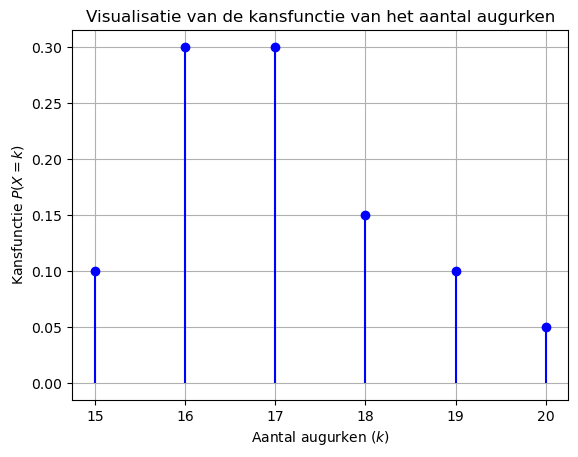
\includegraphics{opg4.4a.png}
            }
        \end{center}
    }

    \item Bereken en teken de cumulatieve kansfunctie. 
    \answer{
        We beschreven $F$, de cumulatieve verdelingsfunctie (CDF), door middel van een tabel:
        \begin{center}
            \begin{tabular}{ccccccc}
                \toprule
                    {\bfseries Aantal augurken $k$} & $15$ & $16$ & $17$ & $18$ & $19$ & $20$\\
                \cmidrule{1-1} \cmidrule{2-2} \cmidrule{3-3} \cmidrule{4-4} \cmidrule{5-5} \cmidrule{6-6} \cmidrule{7-7}
                    $F(k)=P(X \le k)$ & $0,10$ & $0,40$ & $0,70$ & $0,85$ & $0,95$ & $1,00$\\
                \bottomrule
            \end{tabular}
        \end{center}

        In een grafiekvorm ziet dit er als volgt uit:
        
        \begin{center}
            \resizebox{0.9\textwidth}{!}{
                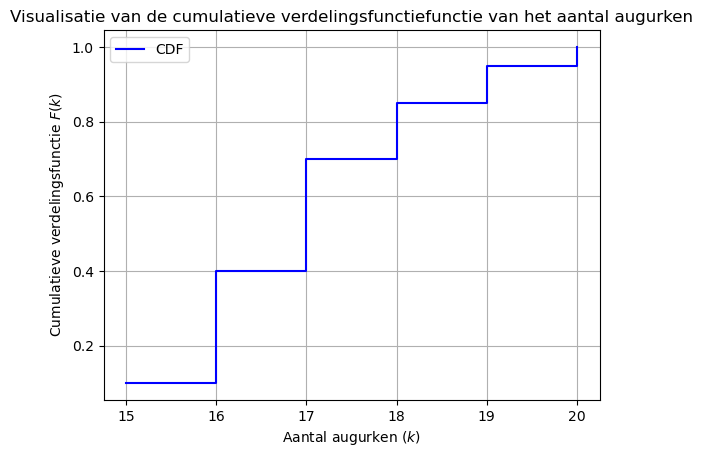
\includegraphics{opg4.4b.png}
            }
        \end{center}
    }

    \item Hoe groot is de kans om in een willekeurige pot meer dan 16 maar minder dan 20 augurken aan te treffen?
    \answer{
        We willen de kans $P(16 < X < 20)$ bepalen. Omdat we met een discrete verdeling werken, kunnen we die als volgt berekenen:
        \[
            P(16 < X < 20) = P(17 \le X \le 19) = F(19) - F(16) = 0,95 - 0,40 = 0,55.
        \]
    }  

    \item Er worden twee willekeurige potten augurken geselecteerd.
    Hoe groot is de kans dat beide potten meer dan 18 augurken bevatten?
    \answer{
        Als er twee willekeurige potten geselecteerd zijn, dan geldt dat beide met kans $P(X > 18) = 1 - P(X \le 18) = 1 - 0,85 = 0,15$ meer dan 18 augurken bevatten.
        Omdat de potten onafhankelijk van elkaar gevuld zijn, is de totale kans gelijk aan $0,15 \cdot 0,15 = 0,0225$.
    }  

    \item Hoe groot is de kans dat twee willekeurige potten augurken in totaal 38 augurken bevatten.
    \answer{
        Laat nu $X_1$ het aantal augurken zijn in pot 1, en $X_2$ het aantal augurken in pot 2.
        We willen de kans $P(X_1+X_2=38)$ bepalen. Dit doen we als volgt:
        \begin{align*}
            P(X_1+X_2=38) &= P(X_1 = 18, X_2=20) + P(X_1 = 19, X_2=19) \\
                          &\qquad + P(X_1 = 20, X_2=18) \\
                          &= 0,15 \cdot 0,05 + 0,10 \cdot 0,10 + 0,05 \cdot 0,15 \\
                          &= 0,025.
        \end{align*}
        Met $2,5\%$ kans is het totaal aantal augurken in twee willekeurige potten samen gelijk aan 38.
    }
    \end{enumerate}

\question{4.6}{Bij een schoolreisje worden vier bussen gebruikt met elk een eigen chauffeur. Van de in totaal 130 leerlingen 
hebben deze bussen respectievelijk 45, 35, 30 en 20 leerlingen vervoerd.}
    
    \begin{enumerate}[label=(\alph*)]
        \item Op basis van toeval kiest men \'e\'en van de vier chauffeurs. Men vraagt aan de chauffeur hoe groot $X$ is, het aantal leerlingen in zijn bus.
        Bereken $E[X]$.
        \answer{
            $X$ is het aantal leerlingen in de bus van een willekeurige chauffeur. De onderliggende kansverdeling is dan
            
            \begin{center}
                \begin{tabular}{ccccc}
                    \toprule
                        {\bfseries Aantal leerlingen $k$} & $20$ & $30$ & $35$ & $45$\\
                    \cmidrule{1-1} \cmidrule{2-2} \cmidrule{3-3} \cmidrule{4-4} \cmidrule{5-5}
                        $P(X=k)$ & $0,25$ & $0,25$ & $0,25$ & $0,25$\\
                    \bottomrule
                \end{tabular}
            \end{center}

            Het is immers zo dat ieder van de vier chauffeurs gekozen wordt met kans $\frac{1}{4}$.
            De verwachtingswaarde $E[X]$ is dan
            \[
               E[X] = \sum_k k \cdot P(X=k) = 20 \cdot 0,25 + 30 \cdot 0,25 + 35 \cdot 0,25 + 45 \cdot 0,25 = 32,5.
            \] 
        }

        \item Op basis van toeval kiest men \'e\'en van de 130 leerlingen en vraagt aan hem of haar hoeveel leerlingen $Y$ er in de bus zaten waarmee deze leerling werd vervoerd.
        Bereken $E[Y]$.
        \answer{
            $X$ is het aantal leerlingen in de bus van een willekeurige leerling. 
            Het totaal aantal leerlingen is $20+30+35+45=130$. 
            De onderliggende kansverdeling is dan
            
            \begin{center}
                \begin{tabular}{ccccc}
                    \toprule
                        {\bfseries Aantal leerlingen $k$} & $20$ & $30$ & $35$ & $45$\\
                    \cmidrule{1-1} \cmidrule{2-2} \cmidrule{3-3} \cmidrule{4-4} \cmidrule{5-5}
                        $P(Y=k)$ & $\frac{20}{130}$ & $\frac{30}{130}$ & $\frac{35}{130}$ & $\frac{45}{130}$\\
                    \bottomrule
                \end{tabular}
            \end{center}

            Het is immers zo dat de kans op een uitkomst evenredig is met het aantal leerlingen dat in een bus met een aantal leerlingen zit.
            De verwachtingswaarde $E[Y]$ is dan
            \[
               E[Y] = \sum_k k \cdot P(Y=k) = 20 \cdot \frac{20}{130} + 30 \cdot \frac{30}{130}  + 35 \cdot \frac{35}{130} + 45 \cdot \frac{45}{130} = 35.
            \]
        }
\end{enumerate}

\question{4.7}{Het aantal personen dat in een willekeurig uur opbelt naar de klantenservice van een groot bedrijf, wordt beschreven door de kansvariabele $X$,
waarvan de gegevens zijn geplaatst in de volgende tabel:}

\begin{center}
    \begin{tabular}{ccccccc}
        \toprule
            {\bfseries Aantal $k$} & $0$ & $1$ & $2$ & $3$ & $4$ & $5$\\
        \cmidrule{1-1} \cmidrule{2-2} \cmidrule{3-3} \cmidrule{4-4} \cmidrule{5-5} \cmidrule{6-6} \cmidrule{7-7}
            {\bfseries $f(k)=P(X=k)$} & $0,20$ & $0,30$ & $0,20$ & $0,15$ & $0,10$ & $0,05$ \\
        \bottomrule
    \end{tabular}
\end{center}

    \begin{enumerate}[label=(\alph*)]
        \item Hoe groot is $P(X\ge 3)$ en $P(X\le 3)$
        \answer{
            We berekenen deze kansen als volgt:
            \begin{align*}
                P(X\ge 3) &= P(X=3) + P(X=4) + P(X=5) \\
                          &= 0,15 + 0,10 + 0,05 = 0,30\\
                P(X\le 3) &= 1 - P(X \ge 4) \\
                          &= 1 - (P(X=4) + P(X=5)) \\
                          &= 1 - (0,10+0,05) \\
                          &= 1 - 0,15 = 0,85 
            \end{align*}
        }

        \item Bereken de verwachtingswaarde van $X$.
        \answer{
            We berekenen de verwachtingswaarde van $X$ als volgt:
            \begin{align*}
                E[X]    &= \sum_k k \cdot P(X=k) \\
                        &= 0 \cdot P(X=0) + 1 \cdot P(X=1) + \ldots + 5 \cdot P(X=5) \\
                        &= 0 \cdot 0,20 + 1 \cdot 0,30 + \ldots + 5 \cdot 0,05 \\
                        &= 1,8
            \end{align*}
        }

        \item Bereken de standaarddeviatie van $X$.
        \answer{
            We berekenen de standaarddeviatie van $X$ door eerst de variantie te berekene:
            \begin{align*}
                Var(X)    &= \sum_k (k-E[X])^2 \cdot P(X=k) \\
                        &= (0-1,8)^2 \cdot P(X=0) + (1-1,8)^2 \cdot P(X=1) + \ldots \\
                        & \qquad + (5-1,8)^2  \cdot P(X=5) \\
                        &= (0-1,8)^2 \cdot 0,20 + (1-1,8)^2 \cdot 0,30 + \ldots + (5-1,8)^2 \cdot 0,05 \\
                        &= 2,06
            \end{align*}

            De standaarddeviatie vinden we dan door de wortel uit de variantie te nemen:
            \[
                \sigma(X) = \sqrt{Var(X)}= \sqrt{2,06} \approx 1,4353
            \]
        }
    \end{enumerate}


\question{4.9}{Een huiseigenaar in Amsterdam besluit drie kamers te huur aan te bieden via Airbnb.
Het dagelijks aantal verhuurde kamers op een willekeurige dag kan worden weergegeven door de kansvariabele $X$, zoals weergegeven in de tabel:}

\begin{center}
    \begin{tabular}{cc}
        \toprule
            {\bfseries Aantal boekingen} & {\bfseries $P(X=k)$}\\
        \cmidrule{1-1} \cmidrule{2-2}
            $0$ & $0,50$ \\
            $1$ & $0,25$ \\
            $2$ & $0,15$ \\
            $3$ & $0,10$ \\
        \cmidrule{1-1} \cmidrule{2-2}
            {\bfseries Totaal} & $1,00$\\
        \bottomrule
    \end{tabular}
\end{center}

    \begin{enumerate}[label=(\alph*)]
        \item Hoe groot is de kans dat op een willekeurige dag minstens twee kamers zijn verhuurd.
        \answer{
            We berekenen deze kans als volgt:
            \begin{align*}
                P(X\ge 2)   &= P(X=2) + P(X=3) \\
                            &= 0,15 + 0,10 \\
                            &= 0,25 \\
            \end{align*}
        }

        \item De aantallen boekingen op twee opeenvolgende dagen kan men beschouwen als onderling onafhankelijke kansvariabelen.
        Maak een kanstabel voor de variabele $X_{\text{som}}$ waarmee het totaal aantal boeking per twee dagen wordt aangegeven.
        Hoe groot is de kans dat in twee dagen meer dan 3 boekingen plaatsvinden?
        \answer{
            De kanstabel voor de somvariabele $X_{\text{som}}$ ziet er als volgt uit:
            \begin{center}
                \begin{tabular}{cc}
                    \toprule
                        {\bfseries Aantal boekingen} & {\bfseries $P(X_{\text{som}}=k)$}\\
                    \cmidrule{1-1} \cmidrule{2-2}
                        $0$ & $0,25$ \\
                        $1$ & $0,25$ \\
                        $2$ & $0,2125$ \\
                        $3$ & $0,175$ \\
                        $4$ & $0,0725$ \\
                        $5$ & $0,03$ \\
                        $6$ & $0,01$ \\
                    \cmidrule{1-1} \cmidrule{2-2}
                        {\bfseries Totaal} & $1,00$\\
                    \bottomrule
                \end{tabular}
            \end{center}
            De kans dat er in twee dagen meer dan 3 boekingen plaatsvinden is dus gelijk aangeeft
            \begin{align*}
                P(X_{\text{som}} > 3)   &= P(X_{\text{som}}= 4) + P(X_{\text{som}}= 5) + P(X_{\text{som}}= 6) \\
                                        &= 0,0725 + 0,03 + 0,01 \\
                                        &= 0,1125
            \end{align*}
        }
\end{enumerate}

\question{4.12}{Een doe-het-zelfzaak verhuurt apparaten waarmee oud behang van een muur kan worden afgestoomd. 
De vraag per dag naar dergelijke apparaten kan worden weergegeven door een kansvariabele $X$ die de volgende waarden aanneemt:}

\begin{center}
    \begin{tabular}{ccccc}
        \toprule
            {\bfseries Aantal gevraagde machines ($k$)} & $0$ & $1$ & $2$ & $3$ \\        
            \cmidrule{1-1} \cmidrule{2-2} \cmidrule{3-3} \cmidrule{4-4} \cmidrule{5-5}
            {\bfseries $P(X=k)$} & $0,20$ & $0,35$ & $0,25$ & $0,20$ \\
        \bottomrule
    \end{tabular}
\end{center}

    \begin{enumerate}[label=(\alph*)]
        \item Bereken de verwachtingswaarde van het aantal gevraagde machines.
        \answer{
            We berekenen deze verwachtingswaarde van het aantal gevraagde machines $X$ als volgt:
            \begin{align*}
                E[X]    &= \sum_k k \cdot P(X=k) \\
                        &= 0 \cdot P(X=0) + \ldots + 3 \cdot P(X=3) \\
                        &= 0 \cdot 0,20 + 1 \cdot 0,35 + 2 \cdot 0,25 + 3 \cdot 0,20 \\
                        &= 1,45
            \end{align*}
        }

        \item De bedrijfsleiding vraagt zich af hoeveel machines in voorraad moeten worden gehouden om aan de (onzekere) vraag te kunnen voldoen.
        Het beschikbaar hebben van zo'n apparaat kost 4 euro per dag, terwijl de huurprijs 6 euro per dag bedraagt.
        Bereken de opbrengst per dag $Y$ indien twee apparaten beschikbaar zijn bij de verschillende waarden van $X$.
        Doe dit ook bij drie beschikbare apparaten. Bereken voor beide gevallen de verwachtingswaarde van $Y$.
        Welke beslissing levert de hoogste verwachtingswaarde. 
        \answer{
            Indien er twee apparaten beschikbaar zijn, beschrijft de volgende tabel de opbrengsten per dag.
            De opbrengsten zijn berekend op basis van opbrengst is huurinkomsten minus beschikbaarheidskosten.

            \begin{center}
                \begin{tabular}{ccccc}
                    \toprule
                        {\bfseries Aantal gevraagde machines ($k$)} & $0$ & $1$ & $2$ & $3$ \\        
                        \cmidrule{1-1} \cmidrule{2-2} \cmidrule{3-3} \cmidrule{4-4} \cmidrule{5-5}
                        {\bfseries Opbrengst $\ell$} & $-8$ & $-2$ & $4$ & $4$ \\        
                        \cmidrule{1-1} \cmidrule{2-2} \cmidrule{3-3} \cmidrule{4-4} \cmidrule{5-5}
                        {\bfseries $P(X=k)$} & $0,20$ & $0,35$ & $0,25$ & $0,20$ \\
                    \bottomrule
                \end{tabular}
            \end{center}
            De verwachte opbrengst bij twee beschikbare apparaten is dus
            \begin{align*}
                E[Y]    &= \sum_\ell \ell \cdot P(X=k) \\
                        &=  -8 \cdot P(X=0) + \ldots + 4 \cdot P(X=3) \\
                        &= -8 \cdot 0,20 + -2 \cdot 0,35 + 4 \cdot 0,25 + 4 \cdot 0,20 \\
                        &= -0,5
            \end{align*}

            Indien er drie apparaten beschikbaar zijn, beschrijft de volgende tabel de opbrengsten per dag.

            \begin{center}
                \begin{tabular}{ccccc}
                    \toprule
                        {\bfseries Aantal gevraagde machines ($k$)} & $0$ & $1$ & $2$ & $3$ \\        
                        \cmidrule{1-1} \cmidrule{2-2} \cmidrule{3-3} \cmidrule{4-4} \cmidrule{5-5}
                        {\bfseries Opbrengst $\ell$} & $-12$ & $-6$ & $0$ & $6$ \\        
                        \cmidrule{1-1} \cmidrule{2-2} \cmidrule{3-3} \cmidrule{4-4} \cmidrule{5-5}
                        {\bfseries $P(X=k)$} & $0,20$ & $0,35$ & $0,25$ & $0,20$ \\
                    \bottomrule
                \end{tabular}
            \end{center}
            De verwachte opbrengst bij twee beschikbare apparaten is dus
            \begin{align*}
                E[Y]    &= \sum_\ell \ell \cdot P(X=k) \\
                        &=  -12 \cdot P(X=0) + \ldots + 6 \cdot P(X=3) \\
                        &= -12 \cdot 0,20 + -6 \cdot 0,35 + 0 \cdot 0,25 + 6 \cdot 0,20 \\
                        &= -3,3
            \end{align*}
            De beslissing om twee apparaten beschikbaar te hebben levert dus naar verwachting de hoogste opbrengst op.
        }
\end{enumerate}

\question{4.13}{In een bedrijf staat een aantal machines opgesteld die soms vanwege een storing moeten worden stilgelegd.
Op grond van ervaring is vastgesteld dat het aantal storingen $X$ per week in de kanstabel wordt beschreven.}

\begin{center}
    \begin{tabular}{cc}
        \toprule
            {\bfseries Aantal storingen ($k$)} & {\bfseries $P(X=k)$} \\        
        \cmidrule{1-1} \cmidrule{2-2}
            $0$ & $0,50$ \\
            $1$ & $0,26$ \\
            $2$ & $0,12$ \\
            $3$ & $0,08$ \\
            $4$ & $0,04$ \\
        \cmidrule{1-1} \cmidrule{2-2}
            Totaal & $1,00$ \\ 
        \bottomrule
    \end{tabular}
\end{center}

    \begin{enumerate}[label=(\alph*)]
        \item Bereken het verwachte aantal storingen per week.
        
        \answer{
            Het verwachte aantal storingen per week berekenen we als volgt:
            \begin{align*}
                E[X]    &= \sum_k k \cdot P(X=k) \\
                        &= 0 \cdot P(X=0) + \ldots + 4 \cdot P(X=4) \\
                        &= 0 \cdot 0,50 + 1 \cdot 0,26 + 2 \cdot 0,12 + 3 \cdot 0,08 + 4 \cdot 0,04 \\
                        &= 0,9
            \end{align*}
        }

        \item Bereken de variantie van het aantal storingen per week.
        \answer{
            Het variantie van het aantal storingen per week berekenen we als volgt:
            \begin{align*}
                Var(X)    &= \sum_k (k-E[X])^2 \cdot P(X=k) \\
                        &= (0-0,9)^2 \cdot P(X=0) + \ldots + (4-0,9)^2 \cdot P(X=4) \\
                        &= (0-0,9)^2 \cdot 0,50 + \ldots + (4-0,9)^2 \cdot 0,04 \\
                        &= 0,81 \cdot 0,50 + \ldots + 9,61 \cdot 0,04 \\
                        &\approx 1,29 
            \end{align*}
        }

        \item Bereken het verwachte aantal storingen per jaar (=50 weken).
        \answer{
            We kunnen het aantal storingen in 50 weken zien als de som $X_{\text{som}}$ van 50 onderling onafhankelijke kansvariabelen $X_1$, $X_2$, \ldots $X_{50}$.
            Aangezien de verwachtingswaarde een lineaire functie is, geldt er dat:
            \begin{align*}
                E[X_{\text{som}}]=E[X_{1} + X_2 + \ldots + X_{50}]    &= E[X_1] + E[X_2] + \ldots + E[X_{50}]\\
                                                    &= 0,9 + 0,9 + \ldots + 0,9 \\
                                                    &= 50 \cdot 0,9 = 45
            \end{align*}
        }

        \item Een storing kost het bedrijf aan reparatie en gemiste productie \euro 500 per geval. Bereken de verwachte storingskosten per jaar.
        \answer{
            De verwachte storingskosten per jaar berekenen we simpelweg door het verwachte aantal storingen per jaar te vermenigvuldigen met de kosten per storing,
            oftewel $45 \cdot $ \euro $500 =$ \euro $22500$.
        }

        \item Bereken de standaarddeviatie van het aantal storingen per jaar.
        \answer{
            Aangezien de wekelijkse aantallen storingen onderling onafhankelijke kansvariabelen zijn, geldt
            \begin{align*}
                Var(X_{\text{som}})     &= Var(X_1 + X_2 + \ldots + X_{50})    \\
                                        &= Var(X_1) + Var(X_2) + \ldots + Var(X_{50}) \\
                                        &= 1,29 + 1,29 + \ldots + 1,29 \\
                                        &= 50 \cdot 1,29 \\
                                        &= 64,5
            \end{align*}

            De standaarddeviatie van het aantal storingen per jaar vinden we door de wortel hiervan te nemen:
            \[
                \sigma(X_{\text{som}}) = \sqrt{Var(X_{\text{som}})} = \sqrt{64,5} \approx 8,03
            \]
        }

    

    \end{enumerate}